\documentclass[]{article}
\usepackage[T1]{fontenc}
\usepackage{lmodern}
\usepackage{amssymb,amsmath}
\usepackage{ifxetex,ifluatex}
\usepackage{fixltx2e} % provides \textsubscript
% use upquote if available, for straight quotes in verbatim environments
\IfFileExists{upquote.sty}{\usepackage{upquote}}{}
\ifnum 0\ifxetex 1\fi\ifluatex 1\fi=0 % if pdftex
  \usepackage[utf8]{inputenc}
\else % if luatex or xelatex
  \ifxetex
    \usepackage{mathspec}
    \usepackage{xltxtra,xunicode}
  \else
    \usepackage{fontspec}
  \fi
  \defaultfontfeatures{Mapping=tex-text,Scale=MatchLowercase}
  \newcommand{\euro}{€}
\fi
% use microtype if available
\IfFileExists{microtype.sty}{\usepackage{microtype}}{}
\usepackage[margin=1in]{geometry}
\usepackage{graphicx}
% Redefine \includegraphics so that, unless explicit options are
% given, the image width will not exceed the width of the page.
% Images get their normal width if they fit onto the page, but
% are scaled down if they would overflow the margins.
\makeatletter
\def\ScaleIfNeeded{%
  \ifdim\Gin@nat@width>\linewidth
    \linewidth
  \else
    \Gin@nat@width
  \fi
}
\makeatother
\let\Oldincludegraphics\includegraphics
{%
 \catcode`\@=11\relax%
 \gdef\includegraphics{\@ifnextchar[{\Oldincludegraphics}{\Oldincludegraphics[width=\ScaleIfNeeded]}}%
}%
\ifxetex
  \usepackage[setpagesize=false, % page size defined by xetex
              unicode=false, % unicode breaks when used with xetex
              xetex]{hyperref}
\else
  \usepackage[unicode=true]{hyperref}
\fi
\hypersetup{breaklinks=true,
            bookmarks=true,
            pdfauthor={Andresa de Andrade},
            pdftitle={Assigment 1},
            colorlinks=true,
            citecolor=blue,
            urlcolor=blue,
            linkcolor=magenta,
            pdfborder={0 0 0}}
\urlstyle{same}  % don't use monospace font for urls
\setlength{\parindent}{0pt}
\setlength{\parskip}{6pt plus 2pt minus 1pt}
\setlength{\emergencystretch}{3em}  % prevent overfull lines
\setcounter{secnumdepth}{5}

\title{Assigment 1}
\author{Andresa de Andrade}
\date{October 4, 2015}

\begin{document}

\begin{center}
\huge Assigment 1 \\[0.2cm]
\end{center}
\begin{center}
\large \emph{Andresa de Andrade}\\[0.1cm]
\end{center}
\begin{center}
\large \emph{October 4, 2015} \\
\end{center}
\normalsize


{
\hypersetup{linkcolor=black}
\setcounter{tocdepth}{2}
\tableofcontents
}
\section{Abstract}\label{abstract}

In recent years, it's become important to understand the factors that
lead a buyer to finalize a conversion within the online marketing
business. Thefore the purpose of this project is to understand any
possible pattern in the customer behavior of an online shop and try to
predict the types of coupons that the customers would want to use/buy.

Along our way we shall demostrante the structure of categorization and
how a machine learning algorithm would work for this particular case. We
will also present the conditions assumed in order to have the model
working properly. And the facts ignored but also important to a
througoly analysis.

We will also show the evaluation methods between the different
methodologies here presented.

\section{Introduction}\label{introduction}

In this paper and the follow documents presented along the way of this
project, we will attempt to demonstrate if the online browsing history
is correlated to final purchase.

In that case, we will be using four data files to learn from. The first
file is composed with the list of 22.874 customers and some personal
information that will be described in the dataset section. The second
file to be used is a file that contains information related to users
buying voucher. And the third file to be used contain the data related
to users browsing in the site. The last file to be used is the coupon
detail information that contains all the data specifically about the
coupon.

\section{Related Research}\label{related-research}

There are several researches and projects done related to online
customer behavior and coupon usage.

\begin{itemize}
\item
  Blattberg et al. (1978) suggested that the coupon usage would be
  related to demographics characteristics where the consumers are
  assumed to minimize the sum of transaction costs, storage costs and
  the price of the item. He basically suggested that the upper income
  households, the more likely to redeem the coupon.
\item
  Narasimhan (1984) proposed that intensity of coupon usage is related
  inversely to a household's opportunity cost of time. Therefore it
  would be expected that in households that are more educated, have
  children under six and husband and wife are employed would have a
  lower prone to use coupons.
\item
  Bawa and W. Shoemaker (1987) suggested that the intention of using the
  coupon (which in their project is called CPI - coupon proneness index)
  is a function of household characteristics and customer behavior.
\end{itemize}

-Kwon Jung (2010) suggested that the online usage of coupon is a funcion
of the percentage of discount offered and demographics.

\section{Dataset}\label{dataset}

As mentioned before, the dataset used is composed by 4 files and they
all have an entity in common. Above you can see the ER diagram for the
data.

\begin{figure}[htbp]
\centering
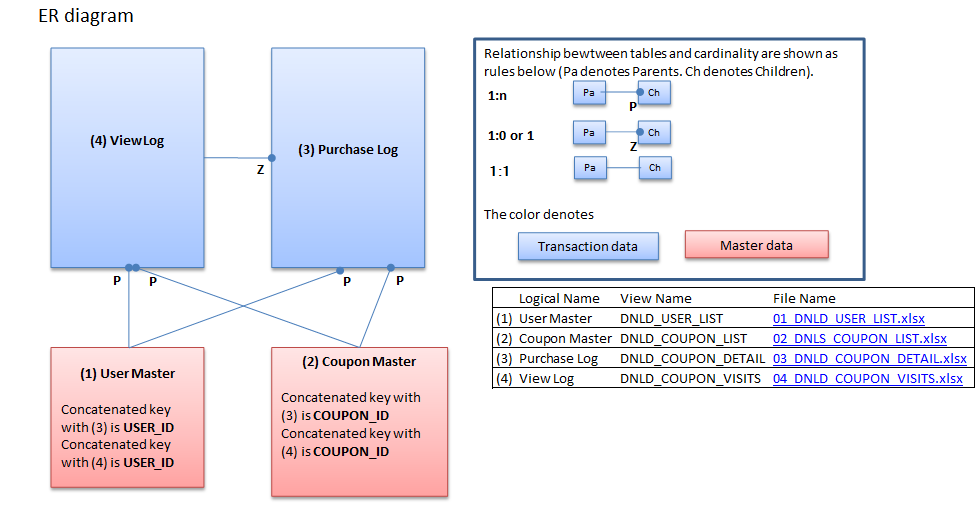
\includegraphics{erdiagram.png}
\caption{ER Diagram}
\end{figure}

\begin{itemize}
\itemsep1pt\parskip0pt\parsep0pt
\item
  user\_list.csv: contains 6 features and 22,873 users. The features are
  related to (registered day, gender, age, date that unregistered,
  preferable name and user id).
\item
  coupon\_detail.csv: contains 6 features and 168,997 entries. The
  columns consist in information about quantity bought, purchase date,
  geographic area that was bought, purchase identifier, user id and
  coupon id.
\item
  coupon\_visits.csv: contains 8 features that refer manly to the
  browsing logs. The columns are purchase flag, purchase id in case it
  happened, log date, page serial, refer, coupon id, user id, session
  id.
\item
  coupon\_list.csv contaisn 24 features related to the coupon like
  category, expire date, what week days it's available, discount value,
  and so on.
\end{itemize}

\section{Analysis}\label{analysis}

In our process to model the data we will have 4 main steps.

\begin{itemize}
\itemsep1pt\parskip0pt\parsep0pt
\item
  Data preparation: where will merge/join the tables creating one single
  table to be used. In addition we will check if there is any missing
  information or data that should be transformed.
\item
  Descriptive Analysis: where we will calculate basic statistics to
  understand how the data is distribuited.
\item
  Modeling: where the methodology will be tested in order to predic the
  coupon usage.
\item
  Data Evaluation: the models will be compared and testes against each
  other in order to choose the best one.
\end{itemize}

\subsection{Data Preparation}\label{data-preparation}

1 - The first step is to merge/ join the browsing history with the user
clients to understand what each client did.

2 - The second is to merge/join the table obtained from 1 to the coupon
details in order to get more clarification of what the coupon offered.

In this way we will have a flatened table with user, browsing, purchase
and coupon information totalizing 44 features.

Because the data comes from Kaggle website, the competion does not share
the purchase log for the test file. Therefore to evaluate the model we
need to separate the dataset in 2 parts: train and test.

Due the reasobable amount of data, we will separated the flatened table
in 80\% for the training and 20\% for the testing and model evaluation.

\subsection{Methodology}\label{methodology}

Looking back at the goal of this project, we need to predict online
coupon usage based on customer behavior.

1 - We will do a descriptive analysis to understand how the data is
distrbuited and if there's any outlier/ pattern that we should be aware
of prior to the

2 - One of the methoodologies very used in the related research is
logistic regression. Basically the response variable would be a dummy
variable considering 1 if the customer used the coupon and 0 otherwise.
The explanatory data would be the customer pattern/behavior.

3 - We will also try to apply Knn methodology to see if there's any
pattern that would helps us to predict the groups of buyers better.

4 - Because the data has a lot of features, it would be interesting to
understand if they are all necessary for the final model. In this case
the methodology PCA will be applied until we reach a 80\% of the
variance explained. Once we have this short data, we will apply n. 2 and
3 and compare the results.

But before any sofisticated methodology, we have to use some descriptive
and sensorial analyses do understand how the data is distributited and
if the hypothesis for the methodology would be respected when we move to
the model.

\subsection{Model Evaluation}\label{model-evaluation}

We will present several models of visualization of the results, being
the confusion of matrix the final evaluation of all the models.

Before and after PCA we will use their main model evaluation to measure
if there's any difference. Being these last ones the pseudo R2, ROC
curve for the logistic regression. And Accuracy being then main criteria
for Knn.

\section{References}\label{references}

\begin{itemize}
\item
  Online vs.~Offline Coupon Redepmtion Behaviors Kwon Jung 2010
\item
  The Coupon Prone Consumer: Some Findings Based on Purchase Behavior
  accross Product Classes.
\item
  Evaluating Logistic Regression at
  \url{http://www.r-bloggers.com/evaluating-logistic-regression-models/}
\item
  Tools for Maching learning at
  \url{http://aimotion.blogspot.ca/2010/08/tools-for-machine-learning-performance.html}
\end{itemize}

\end{document}
